\documentclass[11pt]{article}
\usepackage[utf8]{inputenc}
\usepackage[margin=1in]{geometry}
\usepackage{graphicx}
\usepackage{amsmath, amssymb}
\usepackage{authblk}
\usepackage{hyperref}
\usepackage{natbib}
\usepackage{caption}
\usepackage{booktabs}
\usepackage{float}
\usepackage{graphicx}
\usepackage{subcaption}
\usepackage{float}

\title{Classifying Building Types from Footprints Using Open Geospatial Data and Machine Learning}
\author[1]{Valentin Meo\thanks{ORCID: \href{https://orcid.org/0009-0002-1463-0604}{0009-0002-1463-0604}}}
\affil[1]{Center for Research in Data and Geospatial Intelligence (CRDIG), Université Laval, Québec, Canada\\ \texttt{valentin.meo.1@ulaval.ca}}
\date{March 2023}


\begin{document}

\maketitle

\begin{abstract}
Accurate identification of urban building types is crucial for emergency response planning, particularly during flood events. However, reliable datasets classifying buildings by usage type are scarce, and existing approaches often rely on costly data sources. This study introduces a cost-effective machine learning framework that leverages freely accessible open data—including building footprints, cadastral parcels, road networks, and address points—to classify building types across urban and rural settings in eastern Canada. A comprehensive feature engineering process produced 32 geometric and contextual features. Multiple classifiers were evaluated, with the Random Forest algorithm achieving superior accuracy, reaching up to 96\%in general and correctly identifying up to 99.9\% of residential buildings on a test dataset. This performance surpasses existing approaches and demonstrates high accuracy and practical applicability across diverse regions is possible without expensive data collection—with just simple open data and effective feature engineering. The proposed methodology significantly advances rapid, accurate building classification, facilitating improved emergency response operations.
\end{abstract}

\textbf{Keywords:} Building classification; Machine learning; Open data; Geospatial data; Emergency planning

\section{Introduction}
Information on urban building type is mostly non-existent, yet it is key for many research efforts. This work was part of the ORACLE-2 project. One main goal of this project was to save lives by helping rescuers focus on at-risk residential areas hidden from the road~(\cite{badard2021geomatique}). To achieve this, a reliable building classification dataset was needed. The classification was carried out after building segmentation from satellite imagery and aimed to make it possible to predict the number of settlements in a building and guide rescuers. In this context, this study aimed to use open source data as a way to generate cheap features to predict the building type. To achieve this, many models were tested and optimized. This study was conducted across different eastern Canadian urbanisation types: rural and city.

\section{Previous works}
Recently, governments have tended to provide open and broad access to public data, such as addresses and cadastral parcels, making big data algorithms possible. Despite this, no study has been found that solves the building classification problem using only accessible open data. Indeed, recent studies have shown significant interest in expensive data such as LiDAR as a way to outperform classical topology-based methods~(\cite{wurm2015},~\cite{lloyd2020}). Despite the high precision of LiDAR, these studies failed to provide sufficient accuracy for practical application, especially for predicting minority building types such as industrial and commercial~(\cite{belgiu2014},~\cite{evans2017}), in fact, the method tends to resemble a naive residential prediction relying solely on basic shape data. Moreover, LiDAR is not always available, particularly over large territories. For topology-based methods, accuracy was also insufficient, even when limited to binary classification between residential and non-residential areas~(\cite{wurm2015},~\cite{lloyd2020}). In addition, no study has focused on rural areas, which represent the hardest to classify and the most critical in the event of flooding. Studies have instead focused on residential areas, which are easier to classify. However, considering the limited out-of-distribution generalization capacity of Random Forest—which was the best-performing model—its performance likely does not generalize well to other contexts~(\cite{shimodaira2000covariate}).


\section{Materials and Methods}
\subsection[\appendixname~\thesubsection]{data used:}
Two different areas were selected for the study. The first was a part of Quebec City, representing a typical East Coast urban zone with approximately 50,000 building footprints Figure~\ref{fig:qc}. Quebec is a large, densely urbanized city with an old European-style downtown and a classic North American urban layout, including industrial areas, commercial zones, and suburbs. The second area was the typical North American rural town of Saint-Hyacinthe, along with its surrounding rural sector, comprising approximately 21,000 building footprints Figure~\ref{fig:sh}. The goal of this selection was to represent the diversity of eastern Canadian urbanisation styles. In both datasets, all building types were significantly represented.



\begin{figure}[H]
    \centering
    \begin{subfigure}{0.5\textwidth}
        \centering
        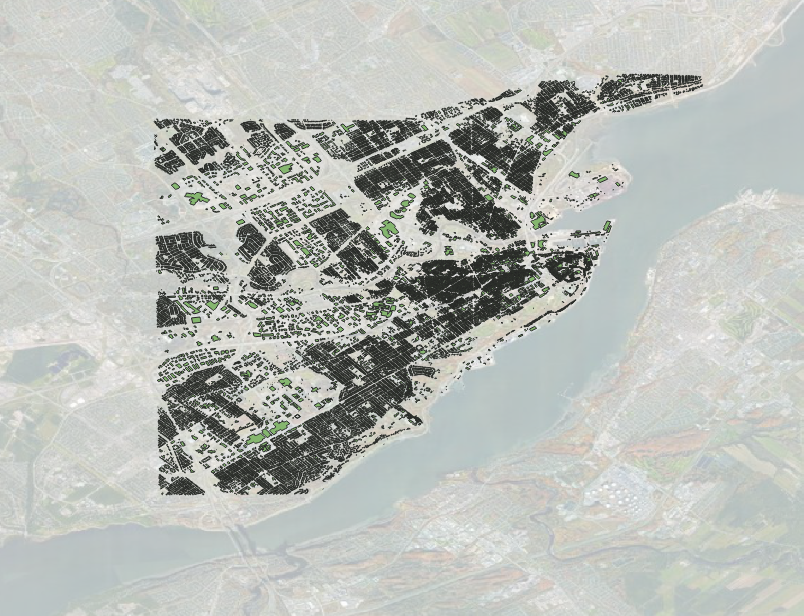
\includegraphics[width=\textwidth]{fig1.png}
       % \caption{}
        %\label{fig:qc-1}
    \end{subfigure}%
    \hfill
    \begin{subfigure}{0.392\textwidth}
        \centering
        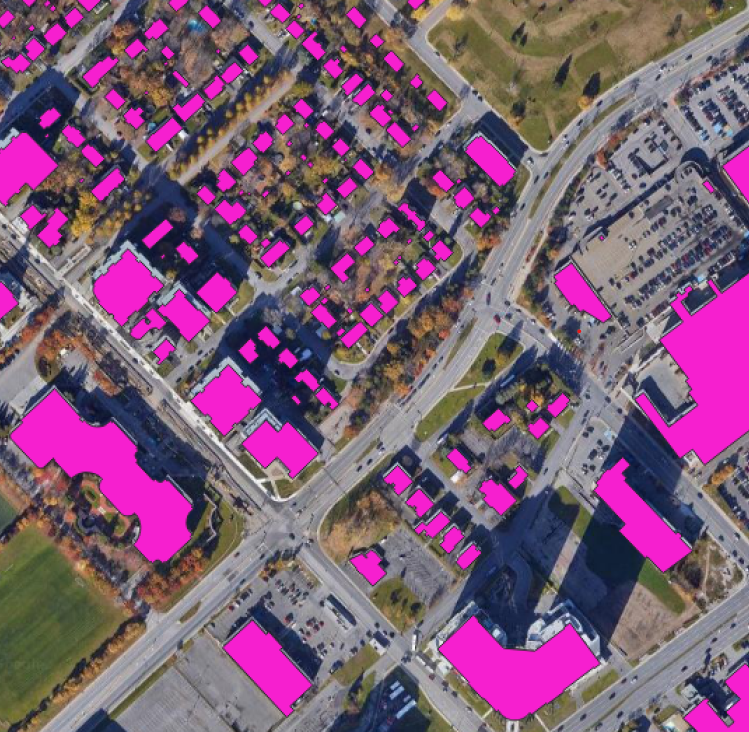
\includegraphics[width=\textwidth]{fig1.2.png}
        %\caption{}
        %\label{fig:qc-2}
    \end{subfigure}
    \captionsetup{justification=centering}
    \caption{Quebec City with building footprints used}
    \label{fig:qc}
\end{figure}

\begin{figure}[H]
    \centering
    \begin{subfigure}{0.5\textwidth}
        \centering
        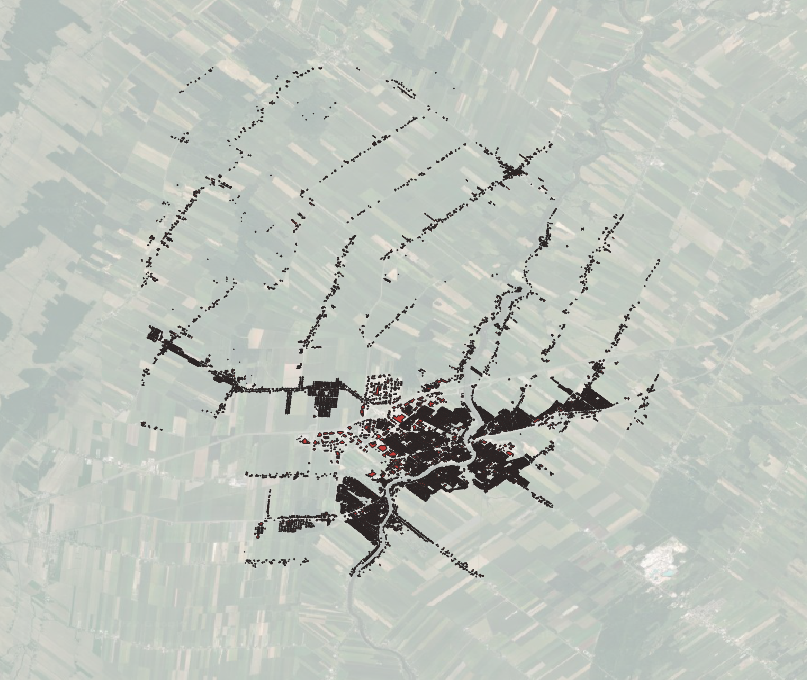
\includegraphics[width=\textwidth]{fig2.png}
       % \caption{}
      %  \label{fig:sh-1}
    \end{subfigure}%
    \hfill
    \begin{subfigure}{0.437\textwidth}
        \centering
        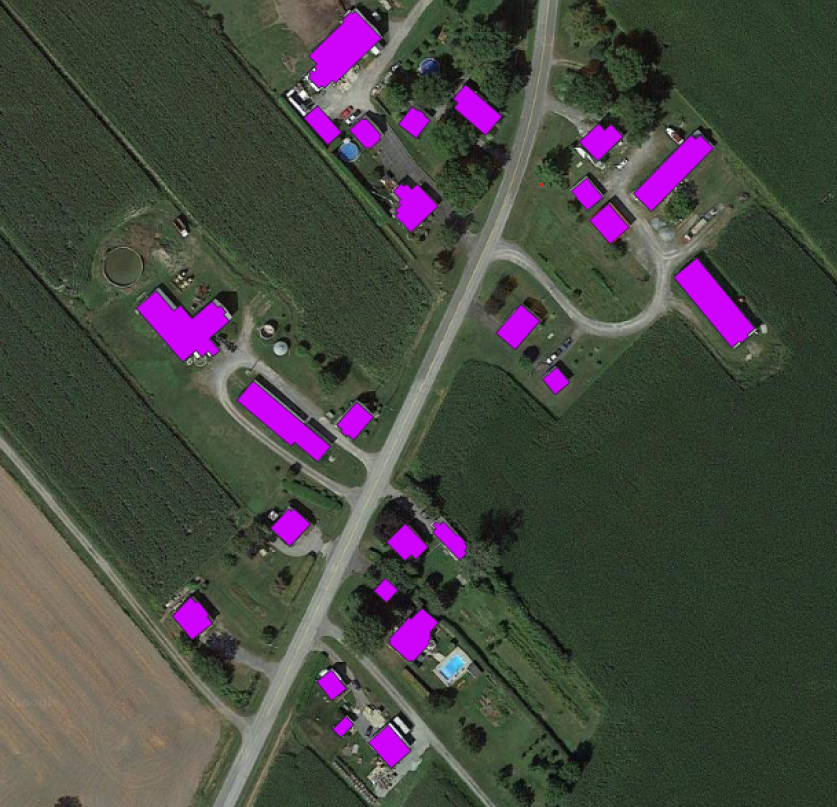
\includegraphics[width=\textwidth]{fig2.2.png}
      %  \caption{}
       % \label{fig:sh-2}
    \end{subfigure}
    \captionsetup{justification=centering}
    \caption{Saint-Hyacinthe with building footprints used}
    \label{fig:sh}
\end{figure}



To enrich the dataset and solve the classification problem, four open datasets were used:

\begin{itemize}
    \item \textbf{Building footprints, altitude}
    
    \item \textbf{Address points} associated with categorical labels. However, the position and category of the addresses were of poor quality. Predicting the closest address category for each building did not outperform the baseline. Despite this, the address category was expected to have a positive impact on the results, as it provides clues about industrial or commercial zones.
    
    \item \textbf{Geometries of cadastral parcels.} Parcels often share common characteristics — for example, in rural areas, there is usually only one residential building per parcel.
    
    \item \textbf{Road networks}, including their geometry, type (street, boulevard, etc.), and hierarchy (interstate, country road, etc.). Indeed information from buildings, addresses, and parcels needed to be contextualized with the surrounding environment. The road dataset was of high quality and enabled such contextualization. For instance, a building located far from a rural path should be interpreted differently than one near an interstate highway.
\end{itemize}

In the case of Quebec City, all data was obtained from the city's open data portal~(\url{https://www.ville.quebec.qc.ca/services/donnees-services-ouverts/index.aspx}). For the rural area, datasets from the provincial government were used~(\cite{villedequebec2025},~\cite{opencanada_qc2025}), except for the building footprints. Although public footprint datasets exist (e.g., Microsoft~:\cite{ms2023globalmlbuildingfootprints}, OpenStreetMap~:\cite{openstreetmap_api2025}), internal produced data from the CRDIG laboratory was preferred due to its easy availability.


All building footprints were manually labeled into the following categories:

\begin{itemize}
    \item Residential
    \item Garage / Garden shed
    \item Agricultural building
    \item Commercial building
    \item Industrial building
    \item Institutional building (church, school, etc.)
\end{itemize}

The distribution of these categories is shown in Figure~\ref{fig:building-distribution}. If a building had two possible types, priority was given to the residential label. Indeed, the ORACLE-2 project aims to identify houses for first responders in the event of flooding.  
This requires ensuring that every building used for living purposes is correctly identified. The most common ambiguous cases involved mixed residential and commercial use.

Buildings that could not be confidently assigned to any of the categories were removed from the dataset. Overdetected footprints—also referred to as detection errors—were likewise removed. These accounted for approximately 1\% of the total buildings.



\begin{figure}[H]
\centering
\begin{subfigure}{0.48\textwidth}
\centering
\caption*{Dataset: Saint-Hyacinthe (Rural)}
\begin{tabular}{lr}
\toprule
Building Type & Number \\
\midrule
Residential & 14,908 \\
Garage / Shed & 2,557 \\
Agricultural Building & 812 \\
Industrial Building & 659 \\
Commercial Building & 410 \\
Institutional Building & 93 \\
\bottomrule
\end{tabular}
\end{subfigure}%
\hfill
\begin{subfigure}{0.48\textwidth}
\centering
\caption*{Dataset: Quebec City (Urban)}
\begin{tabular}{lr}
\toprule
Building Type & Number \\
\midrule
Residential & 33,504 \\
Garage / Shed & 17,553 \\
Agricultural Building & 0 \\
Commercial Building & 1,477 \\
Industrial Building & 630 \\
Institutional Building & 535 \\
\bottomrule
\end{tabular}
\end{subfigure}
\caption{Distribution of building types in both study areas after manual tagging}
\label{fig:building-distribution}
\end{figure}




\subsection[\appendixname~\thesubsection]{Features Engineering:}

During the tagging and exploration phase, several field-based observations were made. In rural areas, residential houses were often closer to and more aligned with roads compared to other buildings. In both urban and rural areas, the address point was usually located at the center of the cadastral parcel. For these reasons, many features were derived based on relationships between buildings, parcels, and roads.

A total of 32 features were computed for each building footprint to support the classification task. These features are grouped below by type:

\paragraph{Footprint Geometry Features}
To capture the specific shape characteristics of certain building types, the following basic geometric features were included:

\begin{itemize}
    \item Surface area of the footprint
    \item Number of vertices
    \item Perimeter
    \item Elongation: ratio between width and height of the minimum bounding rectangle, normalized in [0, 1]
\end{itemize}

\paragraph{Road Context Features}
Since road type and proximity give contextual information, especially about building use, the following features were added:

\begin{itemize}
    \item Generic type of the nearest road (e.g., road, avenue)
    \item Road class (e.g., interstate, country road)
\end{itemize}

\paragraph{Address Features}
Although address data had low positional accuracy, the associated category provided valuable information. Thus:

\begin{itemize}
    \item Category of the nearest address
\end{itemize}

\paragraph{Parcel Features}
Cadastral parcel characteristics were especially relevant in rural settings:

\begin{itemize}
    \item Parcel surface area
    \item Average surface area of adjacent parcels
\end{itemize}

\paragraph{Altitude Feature}
Altitude was observed to influence building type. Industrial zones tend to be near rivers (low altitude), while building at higher elevations are often residential. Therefore:

\begin{itemize}
    \item Median altitude of the building footprint
\end{itemize}

\paragraph{Road-Building Relationship Features}
Some buildings had a specific relationship to the nearest road, like storage buildings or the house that often faced the road in rural areas compared to other buildings. In rural areas, it was observed that the building closest to the road is often the residential building, while in urban areas, the garage was the closest. For this reason, 3 following features were added

\begin{itemize}
    \item Distance to the nearest road
    \item Alignment with the nearest road
    \item Average distance between parcel buildings and the nearest road
\end{itemize}

\paragraph{Address-Parcel Aggregates}
To enrich low-quality address data, per-parcel aggregations were computed:

\begin{itemize}
    \item Count of addresses by category within the parcel
    \item Total number of addresses on the parcel
    \item Most common address category in adjacent parcels
\end{itemize}

\paragraph{Building Count Feature}
The number of buildings on a parcel often relates to its function:

\begin{itemize}
    \item Number of buildings on the parcel
\end{itemize}

\paragraph{Building Context Features}
Contextual features around each building were extracted to model neighborhood patterns:

\begin{itemize}
    \item Average surface of other buildings on the parcel
    \item Number of buildings within a 600-meter buffer. 600 meters were chosen because the number of buildings inside was significant.
    \item Number of buildings within a 50-meter buffer. Because the edge situation of the previous function was not sufficient, we added a closer area.
    \item Average distance between the building and others on the parcel
    \item Average distance between the nearest building and other buildings on the parcel
\end{itemize}

\paragraph{Address-Building Relationship Features}
Given imprecision in address positions, we added features to express spatial relationships:

\begin{itemize}
    \item Distance between the address and the center of the building
    \item Ratio of distances: building to nearest address vs. to the address's nearest building
\end{itemize}

\paragraph{LiDAR Feature}
To better distinguish between condos, industrial, and commercial buildings, a low precision LiDAR-based feature was included:

\begin{itemize}
    \item Median height of LiDAR points over the footprint (using ~30 points per building)
\end{itemize}

\paragraph{Zonal Context Features}
Industrial and institutional buildings often cluster together and exhibit surrounding address patterns. Usually, buildings in this area had the common address category ’Other’ present on the parcel. But the rarest industrial or institutional address category could be observed in the near area outside the parcel. To find this area, the features below were created:

\begin{itemize}
    \item Ratio of number of industrial addresses within 1000 meters to number of buildings in the same area. 1000 was chosen because industrial areas were usually large.
    \item Ratio of number of institutional addresses within 1000 meters to number of buildings in the same area. 1000 was chosen because the institutional cluster was generally not too close to each other, but remained in the same area.
\end{itemize}

\paragraph{Rule-Based Feature (Pseudo-Classifier)}
During data exploration, domain-based logic rules were discovered. For example, if there is one address and one building on a parcel, the address category can be directly assigned. If there are two buildings and one residential address on a small parcel, the smallest building is likely a garage and the other a house. These insights were encoded into a small algorithm using address, road, cadastral, and footprint data. Although this rule-based classifier reached ~80\% accuracy on its own, it was eventually included as an additional feature. Further details are available in the source code.


\subsection[\appendixname~\thesubsection]{Model Selection and Baseline:}


The baseline used in this study was a simple naive prediction: every building is classified as \textit{residential}. This provides a reference point to evaluate whether the machine learning models perform better than chance or naive heuristics.


Several models commonly used in the literature for classification tasks~(\cite{wurm2015},~\cite{lloyd2020}) were selected, along with a few classical algorithms for classification probleme. All models were implemented using the \texttt{scikit-learn} library~(\cite{scikit-learn}).


The models tested are:

\begin{itemize}
    \item \textbf{K-Nearest Neighbors (KNN)} using the Canberra distance metric~(\cite{lance1967canberra}) . During the optimization process, the Canberra metric produced the best results, likely due to the categorical nature of many features.

    
    \item \textbf{Support Vector Classifier (SVC)} — a robust algorithm for high-dimensional classification problems~(\cite{cortes1995svm}).

    \item \textbf{Decision Tree Classifier} — useful for interpretability and feature importance analysis~(\cite{quinlan1986id3}).

    
    \item \textbf{Multi-layer Perceptron (MLP)} — a simple feedforward neural network~(\cite{rumelhart1986mlp}).



    \item \textbf{Random Forest Classifier} — a widely used ensemble method based on decision trees~(\cite{breiman2001randomforest}).

    
    \item \textbf{Gradient Boosting Classifier} — a powerful boosting-based ensemble method~(\cite{friedman2001gradient}).

\end{itemize}

Random Forest was expected to outperform the other models, as supported by findings in the literature~(\cite{lloyd2020}).


\section{Results}
\subsection[\appendixname~\thesubsection]{Base line:}
\par
The base line gives an accuracy of 0.726 for the urban area and 0.642 for the rural area.
\par


\subsection[\appendixname~\thesubsection]{Results of the different models:}
\par
Figure~\ref{fig:results-rural-table} shows the performance of different models on the rural area test dataset.  
The best-performing model was the Random Forest, with its corresponding confusion matrix presented in Figure~\ref{fig:results-rural-confusion}. Figure~\ref{fig:results-urban} shows the results for the urban area test dataset. Random Forest was again the best-performing model, and its confusion matrix is presented in the same figure.

\par
\begin{figure}[H]
\centering
\begin{subfigure}{0.48\textwidth}
\centering
\begin{tabular}{lc}
\toprule
Model & Result \\
\midrule
K-Nearest Neighbors (KNN) & 0.9445 \\
Support Vector Classifier (SVC) & 0.9519 \\
Decision Tree & 0.9309 \\
Multi-Layer Perceptron (MLP) & 0.9473 \\
Random Forest & 0.9604 \\
Gradient Boosting & 0.9563 \\
\bottomrule
\end{tabular}
\caption{Model accuracy on rural area}
\label{fig:results-rural-table}
\end{subfigure}%
\hfill
\begin{subfigure}{0.48\textwidth}
\centering
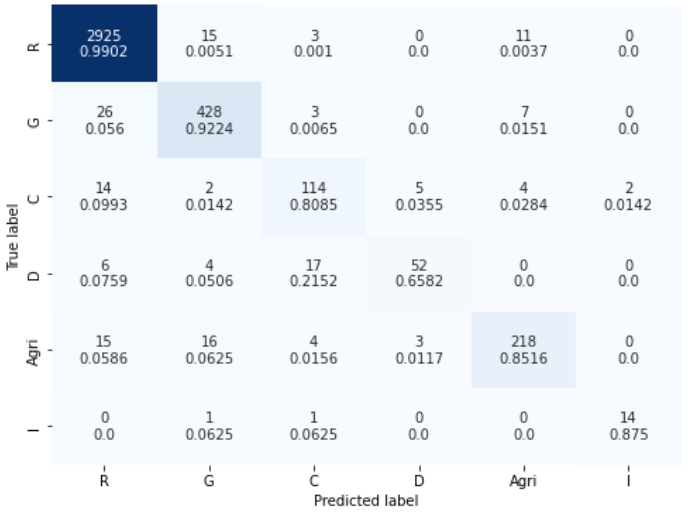
\includegraphics[width=\linewidth]{fig6.png}
\caption{Confusion matrix of Random Forest on rural area}
\label{fig:results-rural-confusion}
\end{subfigure}
\caption{Model evaluation on rural area: (a) accuracy comparison, (b) Random Forest confusion matrix.}
\label{fig:results-rural}
\end{figure}



\begin{figure}[H]
\centering
\begin{subfigure}{0.48\textwidth}
\centering
\begin{tabular}{lc}
\toprule
Model & Result \\
\midrule
K-Nearest Neighbors (KNN) & 0.9625 \\
Support Vector Classifier (SVC) & 0.9632 \\
Decision Tree & 0.9484 \\
Multi-Layer Perceptron (MLP) & 0.9610 \\
Random Forest & 0.9687 \\
Gradient Boosting & 0.9640 \\
\bottomrule
\end{tabular}
\caption{Model accuracy on urban area}
\label{fig:results-urban-table}
\end{subfigure}%
\hfill
\begin{subfigure}{0.48\textwidth}
\centering
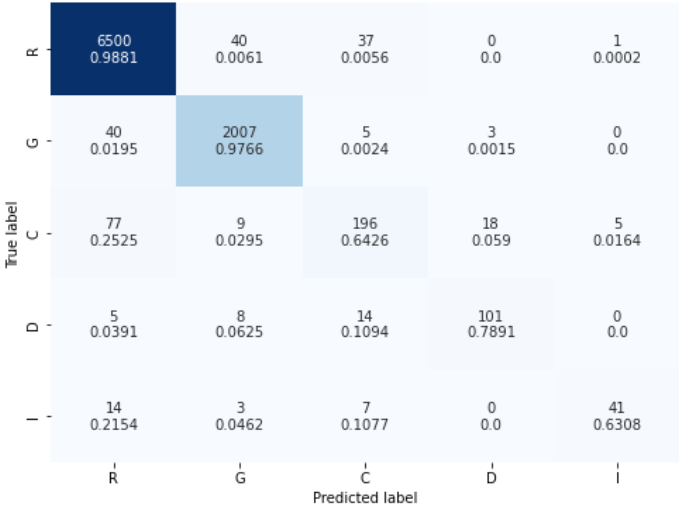
\includegraphics[width=\linewidth]{fig8.png}
\caption{Confusion matrix of Random Forest on urban area}
\label{fig:results-urban-confusion}
\end{subfigure}
\caption{Model evaluation on urban area: (a) accuracy comparison, (b) Random Forest confusion matrix.}
\label{fig:results-urban}
\end{figure}





The Random Forest model trained on the rural dataset achieved an accuracy of 0.95 when evaluated on the entire urban dataset. This result demonstrates the robustness and generalizability of the model across different spatial contexts. The reverse experiment—training on urban data and testing on rural data—was not feasible due to the absence of agricultural buildings in the urban dataset.



\section{Discussion :}

According to the literature, Random Forest was generally the most accurate model~(\cite{lloyd2020}).  However, it presented some weaknesses in our specific context. Random Forest is known to underutilize correlated features~(\cite{gregorutti2017correlation}), and in our dataset, many features were indeed correlated. Additionally, Random Forest has limited out-of-distribution generalization capacity, making it less robust across varying data environments~(\cite{rshimodaira2000covariate}).  In our case, the Random Forest score was relatively close to that of other models, which contrasts with previous studies~(\cite{lloyd2020}). This suggests that the feature engineering method used here was robust enough to yield good results across all models tested.





A relatively high confusion was observed between the \textit{industrial} and \textit{commercial} categories, often due to overlapping usage. For instance, some industrial buildings also hosted commercial shops. Labeling such edge cases proved difficult.

Confusion between \textit{residential} and \textit{commercial} buildings was also observed, as many commercial activities occurred within residential buildings. Given the importance of identifying residential buildings in emergency contexts (in our case flooding), the classification strategy prioritized minimizing errors in the residential class. However, this logic sometimes led to misclassifications at category boundaries that were hard to predict.

There was also a high rate of confusion between the \textit{garage} and \textit{residential} categories. Furthermore, a significant drop in performance was observed for identifying commercial buildings in urban areas, primarily due to low-quality address data. In the urban dataset, many \textit{commercial} addresses were found on residential buildings and vice versa, affecting classification accuracy.

The categorization methodology showed a major flaw: while true positives for residential buildings reached up to 99\%, this came at the expense of lower accuracy in other categories. To improve results, a re-categorization process is needed, possibly with the addition of intermediate or related categories.

A feature importance analysis was conducted and is presented in Figure~\ref{fig:fig9} for urban areas and Figure~\ref{fig:fig10} for rural areas. Per-class feature importances are shown in Figure~\ref{fig:fig11} (rural) and Figure~\ref{fig:fig12} (urban).

\begin{figure}[H]
\centering
\begin{subfigure}{0.48\textwidth}
    \centering
    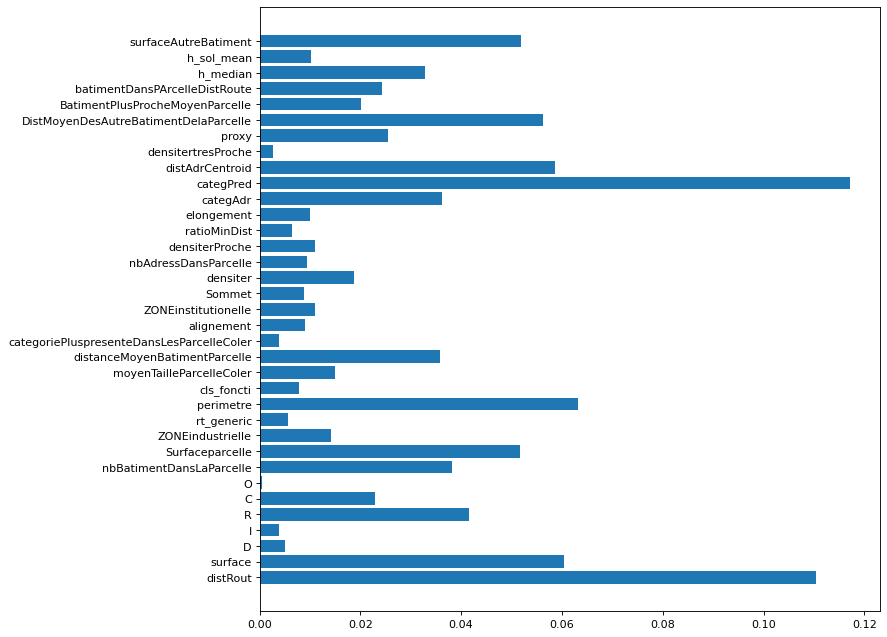
\includegraphics[width=\linewidth]{fig9.png}
    \caption{Feature importance — urban area}
    \label{fig:fig9}
\end{subfigure}%
\hfill
\begin{subfigure}{0.48\textwidth}
    \centering
    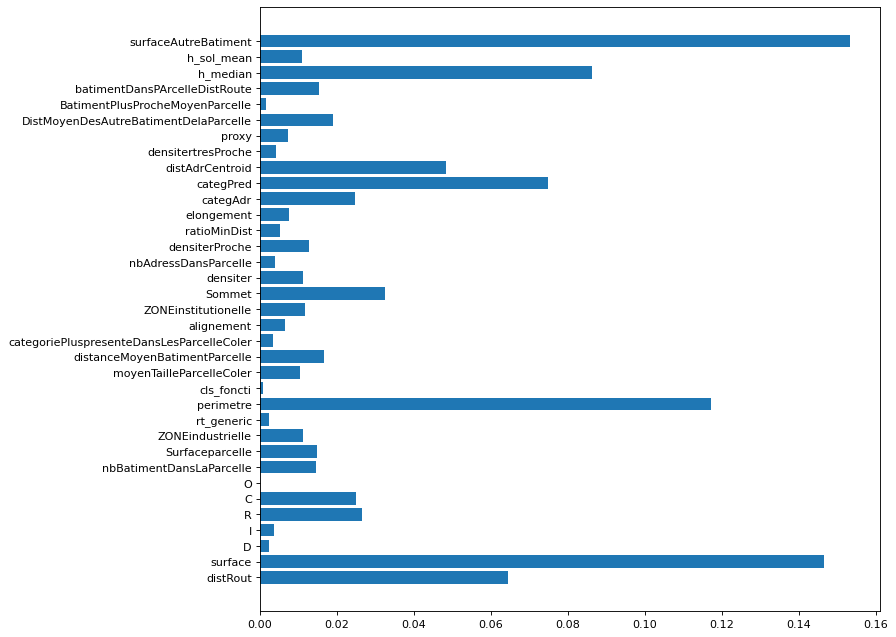
\includegraphics[width=\linewidth]{fig10.png}
    \caption{Feature importance — rural area}
    \label{fig:fig10}
\end{subfigure}

\vspace{0.5cm}

\begin{subfigure}{0.48\textwidth}
    \centering
    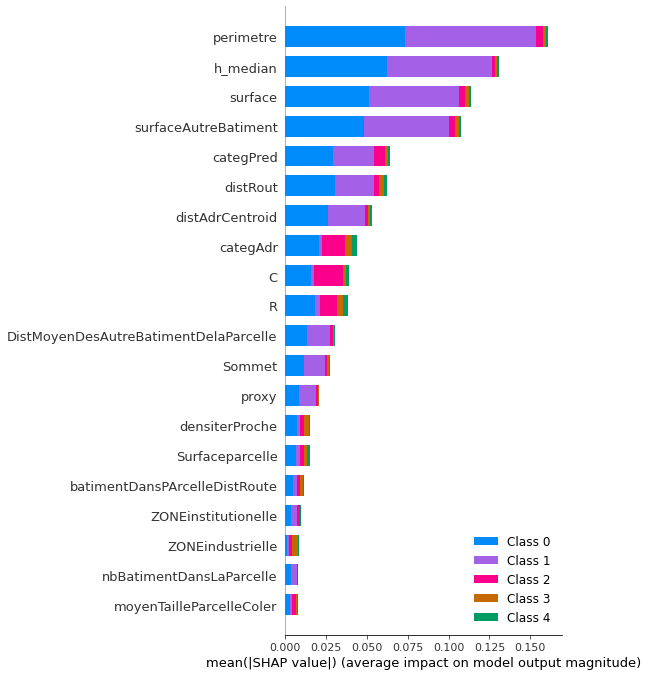
\includegraphics[width=\linewidth]{fig11.png}
    \caption{Per-class feature importance — rural}
    \label{fig:fig11}
\end{subfigure}%
\hfill
\begin{subfigure}{0.48\textwidth}
    \centering
    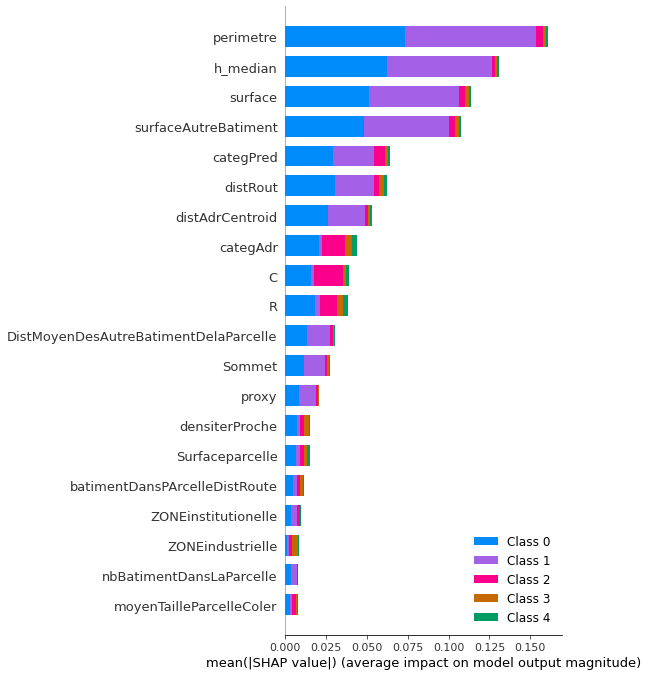
\includegraphics[width=\linewidth]{fig12.png}
    \caption{Per-class feature importance — urban}
    \label{fig:fig12}
\end{subfigure}

\caption{Feature importance analysis across urban and rural datasets}
\label{fig:feature-importance}
\end{figure}



Figures~\ref{fig:fig12} and~\ref{fig:fig11} show that geometric features were the most important overall. Address-related features were less informative than expected, likely because the address position often did not match the building's true location. In addition, many address categories contained errors. Nonetheless, all data sources contributed usefully to the classification.  

One feature of note was the \texttt{h-ground} feature, which showed a significant impact. However, due to the small number of industrial area in the dataset, it is difficult to draw firm conclusions — the effect may reflect overfitting. For example, Quebec City includes a residential hill and an industrial waterfront. But typically, industrial buildings are not located at high altitudes, which give hope for generalisation posibility.

The qualitative error analysis led us to believe that we were approaching the upper bound of prediction precision. During manual labeling, some building types could not be confidently identified using GIS data alone, and OpenStreetMap imagery was required. The source code includes data for performing such qualitative analysis.

\section{Conclusion}

The final model successfully outperformed previous approaches in the literature, while requiring less processing time and using only free and publicly available data. Moreover, our method is applicable to the entire territory of Quebec (rural and urban). The analysis of errors showed that it is difficult to achieve significantly better performance using only this type of data. However, unlike prior studies, the achieved accuracy was sufficient for practical applications involving a diverse range of building types.

To further improve these results, several directions can be considered. First, the use of cadastral zoning information (the cadastral role) could enhance prediction. This dataset, which is freely available, includes urbanization zones, and could help since industrial buildings are not legally allowed in residential areas. Second, while hight presision LiDAR features or image-based inputs could improve accuracy, relying on them would limit the applicability of the method to smaller areas, contrary to the objectives of the ORACLE-2 project, which aims to be used across all of Quebec.

Another promising direction would be to apply convolutional neural networks to analyze the surrounding environment of each building, possibly by integrating aerial or satellite imagery. In addition, a cascaded model approach could be explored, where the first model’s output feeds into a second classifier. This could help improve the understanding of spatial context, such as distinguishing whether a parcel contains a single house, and adjusting the final classification accordingly. Indeed, the second classification had access to the last classification carried out to have a better vision of the context of each building and could adapt the prediction with this extra data.















\section*{Data and Code Availability}

The source code and a subset of the data used in this study are publicly available on GitHub at the following address:  
\url{https://github.com/valkenzz/building-type-predictor}

Due to size and access limitations, the full dataset used for training and evaluation is not hosted online, but can be provided by the authors upon reasonable request.


\section*{Acknowledgments}
The authors would like to thank Thierry Badard for his support.

\section*{Funding}
This work was supported by the ORACLE-2 project.

\section*{Conflict of Interest}
The author declares no conflict of interest.


\bibliographystyle{plainnat}
\bibliography{references}

\end{document}
